\chapter{EMBOSS}

\section{EMBOSS简介}

EMBOSS为整合了多个生物信息学软件的软件包(软件包主页\textit{http://emboss.open-bio.org}),其作者为以Peter Rice为领导的来自欧洲生物信息学研究所的团队。

EMBOSS包含多种功能的生物信息学工具,如基于Needleman-Wunsch动态规划算法的全局比对程序needle,
基于Smith-Waterman算法的局部比对程序water等。

EMBOSS有三种常见的运行方式:命令行界面、图形界面、浏览器界面。
其中,浏览器界面依赖于通过互联网访问装有EMBOSS的服务器进行;图形界面、命令行界面主要依赖于Linux系统完成。
本小节以命令行界面演示代码为主,参数式运行所有命令。

\section{软件功能实例}
\subsection{needle}

needle程序用于两序列的全局比对。以人类CEAM3、CEAM4蛋白质序列比对为例,使用needle程序进行分析:

\begin{lstlisting}
    #! /bin/usr
    path="/rd1/home/public/EMBOSS/input"
    needle ${path}/CEAM3_HUMAN.FASTA ${path}/CEAM4_HUMAN.FASTA CEAM3-GEAM4.NEEDLE -gapo 20 -gape 2
\end{lstlisting}

\begin{quotation}
    -gapo: 起始空位罚分,默认为10。

    -gape: 延伸空位罚分,默认为0.5。
\end{quotation}

CEAM3、CEAM4序列:

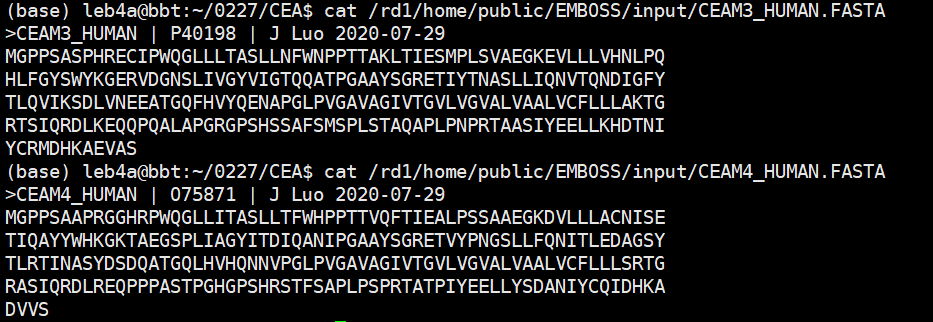
\includegraphics[width=0.8\textwidth]{./image/gdk/5.2.1.png}

输出结果:

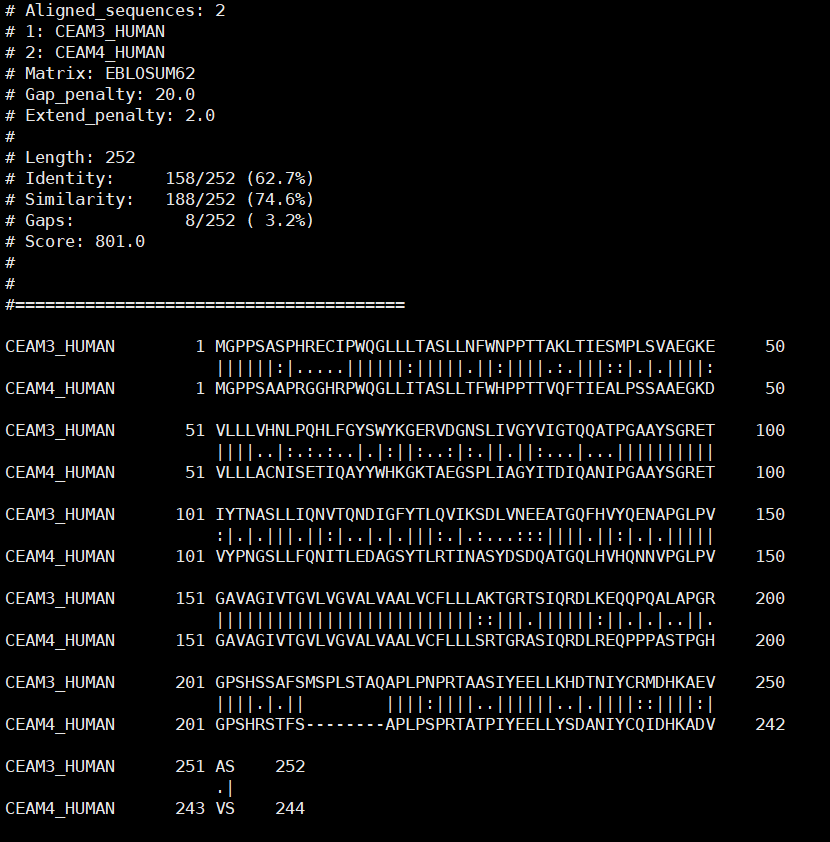
\includegraphics[width=0.8\textwidth]{./image/gdk/5.2.2.png}

\subsection{water}

water程序用于序列的局部比对。以人类CEAM3、、CEAM5蛋白质序列比对为例,使用water程序进行分析:

\begin{lstlisting}
    #! /bin/usr
    path="/rd1/home/public/EMBOSS/input"
    water ${path}/CEAM3_HUMAN.FASTA -sbegin 35 -send 142  \
	    ${path}/CEAM5_HUMAN.FASTA -sbegin 35 -send 142 \
	    ./CEAM3-CEAM5.WATER -gapo 20 -gape 2
\end{lstlisting}

\begin{quotation}
    -sbegin: 比对起始位点。

    -send: 比对终止位点。

    -gapo: 起始空位罚分,默认为10。

    -gape: 延伸空位罚分,默认为0.5。
\end{quotation}

CEAM3、CEAM5序列:

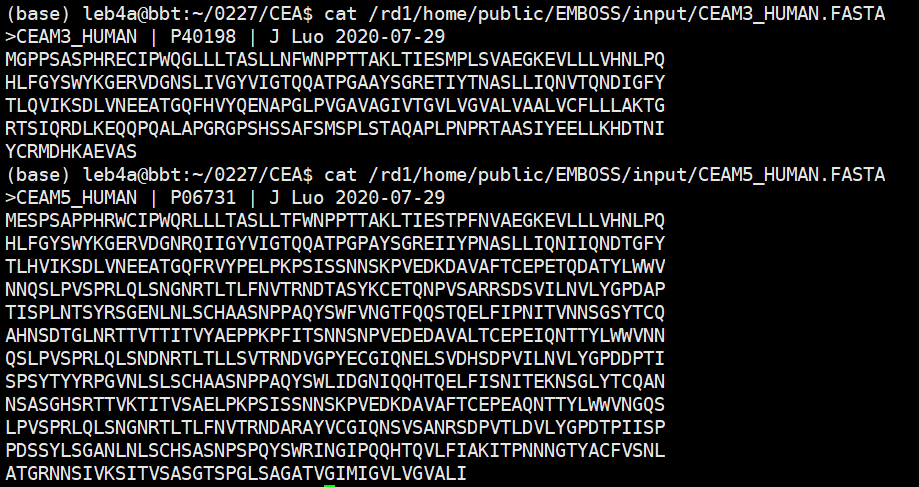
\includegraphics[width=0.8\textwidth]{./image/gdk/5.2.3.png}

输出结果:

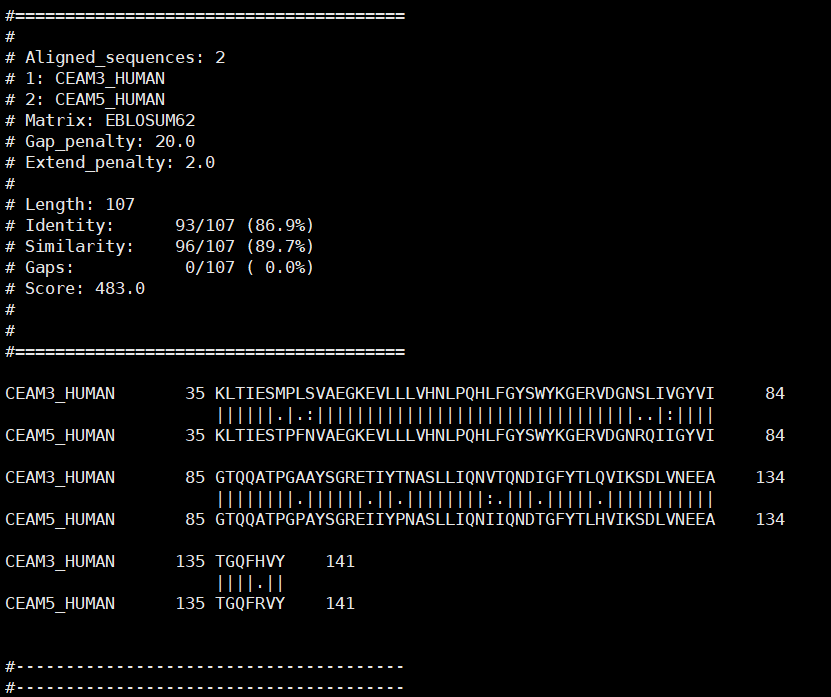
\includegraphics[width=0.8\textwidth]{./image/gdk/5.2.4.png}

\subsection{edialign}

edialign程序用于序列的多重比对。以人类所有CEA蛋白质序列比对为例,使用edialign程序进行分析:

\begin{lstlisting}
    #! /bin/usr
    path="/rd1/home/public/EMBOSS/input"
    edialign ${path}/12HUMAN_CEA.FASTA 12HUMAN_CEA.EDIA 12HUMAN_CEA.ALN
\end{lstlisting}

12个人类CEA氨基酸序列:

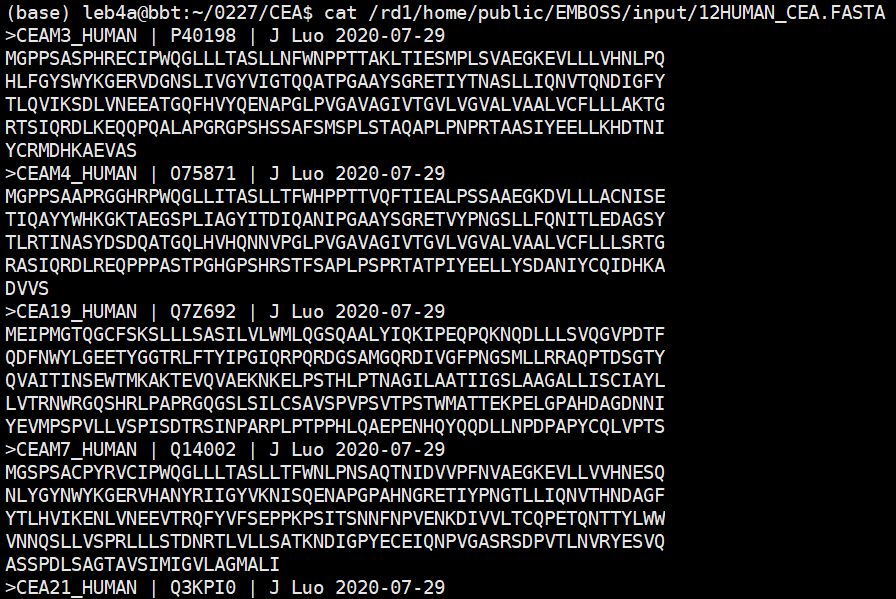
\includegraphics[width=0.8\textwidth]{./image/gdk/5.2.5.png}

部分输出结果:

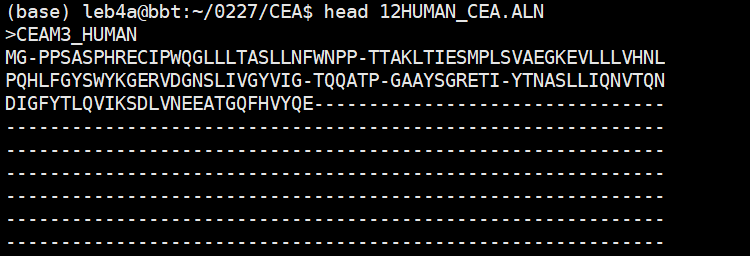
\includegraphics[width=0.8\textwidth]{./image/gdk/5.2.6.png}

\section*{参考资料}
[1]罗静初.EMBOSS和EMBnet[J].生物信息学,2021,19(04):223-231.

[2]罗静初.EMBOSS软件包序列分析程序应用实例[J].生物信息学,2021,19(01):1-25.